\pagebreak
\section{Calcolo integrale per funzioni di più variabili (secondo Riemann)}
\subsection{Introduzione}
\footnote{Slide 12 PDF 24.} Sarà trattato il calcolo integrale per funzioni di 2 variabili, quindi integrali doppi (in quanto il dominio considerato sarà un sottoinsieme del piano). Sarà trattato come gli integrali doppi diventino semplici, cosicché un integrale doppio possa essere trasformato in un integrale iterato, potendo così integrare prima rispetto ad una o poi rispetto all'altra variabile.\\
In particolare, saranno trattate le regole per il cambiamento di variabile degli integrali in coordinate polari (concetto legato ai domini che presentano simmetrie). Ad esempio: tramite l'utilizzo delle coordinate polari un dominio che è un cerchio sul piano cartesiano si trasformerà in un rettangolo nel piano polare.\\
Nell'integrazione multipla secondo Riemann saranno trattati:
\begin{enumerate}
	\item Funzioni Riemann integrabili su opportuni domini (semplici e loro unione opportuna) del piano \footnote{Saranno considerati domini limitati e abbastanza regolari per avere una funzione continua e quindi integrabile su tale dominio.},
	\item Integrali doppi
	\begin{itemize}
		\item Calcolo integrali doppi come prodotto di integrali semplici
		\begin{enumerate}
			\item Formula di riduzione (tramite il Teorema \ref{th:riduzione} di riduzione),
			\item Cambiamento di variabile.
		\end{enumerate}	
		\item Insieme misurabile: misura (area) di un insieme limitato e simmetrico secondo Peano-Jordan.
	\end{itemize}
\end{enumerate}

\subsection{Integrale doppio per funzioni limitate su rettangoli}
\footnote{Slide 13 PDF 24.}
Considerato $R=[a,b]\times[c,d]\subset \mathbb R^2$ (base $\times$ altezza) rettangolo nel piano, dove $R$ è un sottoinsieme del piano chiuso e limitato, è possibile "sezionare" $R$ in sottoinsiemi $R_{ij}\subset R$, a loro volta rettangoli (vedere Figura \ref{fig:rettangolo}).

\begin{figure}[ht]
	\centering
	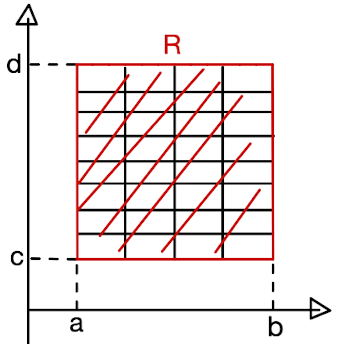
\includegraphics[width=0.35\textwidth]{Analisi2/figures/rettangolo.png}
	\caption{Rettangolo e sottoinsiemi.}
	\label{fig:rettangolo}
\end{figure}

\paragraph{Nota sulla Figura \ref{fig:rettangolo}:}

\paragraph{Nota (non importante):} I rettangolini sono formati creando una partizione di $[a,b]$ e di $[c,d]$ come quella di Calcolo Numerico: ogni intervallo sarà diviso in $n$ sottointervalli di ampiezza $(b-a)/n$ e $(d-c)/n$, mediante l'utilizzo di $n+1$ punti equidistanziati del tipo
\begin{equation*}
	\begin{matrix}
		x_h = a + h \frac{b-a}{n},\quad h=1, \hdots, n,\\\\
		a=x_0<x_1<\hdots<x_n=b
	\end{matrix}
\end{equation*}
oppure 
\begin{equation*}
	\begin{matrix}
		y_k = a + k \frac{b-a}{n},\quad k=1, \hdots, n,\\\\
		c=y_0<y_1<\hdots<y_n=d
	\end{matrix}
\end{equation*}

\paragraph{Nota:} Nel caso generale è possibile utilizzare pluri-intervalli, cioè un prodotto cartesiano di $n$ intervalli. $\qed$

\begin{definition}[Partizione (suddivisione)]
	\footnote{Slide 13 PDF 24.} Sia $R = [a,b]\times [c,d]\subset\mathbb{R}^2$ un rettangolo. Date $D_1$ e $D_2$ due suddivisioni (partizioni) di $[a,b]$ e $[c,d]$ rispettivamente:
	\begin{equation*}
		\begin{matrix}
			D_1 \overset{\footnotemark}{=} \{a = x_0, x_1,\hdots, x_n = b\;|\; \overbrace{x_0<x_1<\hdots <x_n}^{n+1\text{ punti}}\},\quad\text{con } x_i\in[a,b],\\
			D_2 \underset{\footnotemark}{=} \{c=y_0, y_1,\hdots, y_m =d\; | \; \underbrace{y_0<y_1<\hdots<y_n}_{m+1\text{ punti}}\},\quad\text{con } y_s\in[c,d],
		\end{matrix}
	\end{equation*}
	una partizione (suddivisione) del rettangolo $R$ è definita come
	\begin{equation}\label{eq:suddivisione_rettangolo}
		D=D_1\times D_2.
	\end{equation}
\end{definition}
\addtocounter{footnote}{-1}
\footnotetext{Divisione dell'intervallo $[a,b]$ in $n$ intervalli piccoli.}

\stepcounter{footnote}
\footnotetext{Divisione dell'intervallo $[c,d]$ in $n$ intervalli piccoli.}

\paragraph{Nota:} Nella Definizione di Partizione sono considerate due suddivisioni dei due intervalli, ma il loro numero è arbitrario. Il prodotto cartesiano delle suddivisioni dei due intervalli forma una suddivisione del rettangolo $R$, quindi una suddivisione di un rettangolo è l'unione di rettangolini.\\
In corrispondenza di ogni suddivisione degli intervalli $[a,b]$ e $[c,d]$ è possibile definire una suddivisione del rettangolo $R$. Quindi, $R$ è l'unione degli $n\times m$ rettangoli $R_{ij}$, dove
\begin{enumerate}
	\item $D_1$ suddivide $[a,b]$ negli intervalli $[x_{i-1}, x_i]=I_i$, $i=1,\hdots, n$,
	\item $D_1$ suddivide $[c,d]$ negli intervalli $[y_{i-1}, y_j]=J_j$, $j=1,\hdots, m$,
	\item $R_{ij} = [x_{i-1}, x_i] \times [y_{i-1}, y_j] = I_i \times J_j, \; i=1,\hdots, n, j=1,\hdots, m$.
\end{enumerate} $\qed$

\begin{definition}[Estremo superiore e inferiore]
	Considerata $f:R = [a,b]\times[c,d]\rightarrow\mathbb{R}$ limitata,
	\begin{equation*}
		m\leq f(x,y)\leq M,\quad \forall(x,y)\in R,
	\end{equation*}
	e $D_1,D_2$ e $R_{ij}$ definiti come sopra. Per $i=1,\hdots, n$ e $j=1,\hdots, m$, sono definiti estremo inferiore ed estremo superiore di ogni $R_{ij}$ come
	\begin{equation}\label{eq:estremo_inf_sup}
		\begin{matrix}
			m_{ij} := \underset{R_{ij}}{\inf} f\quad\left(\equiv\underset{(x,y)\in R_{ij}}{\inf} f(x,y)\right),\\\\
			M_{ij} := \underset{R_{ij}}{\sup} f\quad\left(\equiv\underset{(x,y)\in R_{ij}}{\sup} f(x,y)\right).
		\end{matrix}
	\end{equation}
	($m_{ij}, M_{ij}$ sono numeri finiti)
\end{definition}

\paragraph{Nota su (\ref{eq:estremo_inf_sup}):} Per ogni rettangolo $R_{ij}$ è presente l'estremo inferiore e superiore perché $f$ è limitata al rettangolo $R_{ij}$. $\qed$

\begin{definition}[Somma inf/superiore]\footnote{Slide 15 PDF 24.}
	Sia $f:R = [a,b]\times[c,d]\rightarrow\mathbb{R}$, $D = D_1\times D_2$ suddivisione di $R$, la somma inferiore è definita come
	\begin{equation*}
		s(f,D) = \sum_{i=1}^{n}\sum_{j=1}^{m} m_{ij} \underbrace{\overbrace{(x_i-x_{i-1})}^{\text{amp.}[x_i-x_{i-1}]} \overbrace{(y_i-y_{i-1})}^{\text{amp.}[y_i,y_{i-1}]}}_{Area(R_{ij})}
	\end{equation*}
	e la somma superiore come
	\begin{equation*}
		S(f,D) = \sum_{i=1}^{n}\sum_{j=1}^{m} M_{ij} (x_i-x_{i-1})(y_i-y_{i-1}).
	\end{equation*}
\end{definition}


\begin{remark}
	Considerata $f:R = [a,b]\times[c,d]\rightarrow\mathbb{R}$ limitata, è possibile osservare che per ogni suddivisione $D$ di $R$ vale
	\begin{equation}\label{eq:limitazione_somme_inf_sup}
		m(b-a)(d-c) \leq s(f, D) \leq S(f, D) \leq M(b-a) (d-c),
	\end{equation}
	dove
	\begin{equation*}
		m\leq f(x,y) \leq M.
	\end{equation*}
\end{remark}

\paragraph{Nota su (\ref{eq:limitazione_somme_inf_sup}):} (\ref{eq:limitazione_somme_inf_sup}) afferma che le somme inferiori sono superiormente limitare e che le somme superiori sono inferiormente limitate al variare di $D$ in tutte le possibili suddivisioni degli intervalli $[a,b], [c,d]$. Inoltre, tutti i membri delle disuguaglianze sono numeri finiti.

\paragraph{Nota:} Al variare di $D$ nell'insieme di tutte le suddivisioni di $R$ (ottenute facendo variare le suddivisioni dei singoli intervalli $[a,b], [c,d]$) risultano ben definite (ovvero sono quantità finite)
\begin{equation*}
	\underset{D}{\sup} s(f,D)\quad\text{e}\quad \underset{D}{\inf} S(f,D),
\end{equation*}
ovvero l'estremo superiore delle somme inferiori e l'estremo inferiore.\\
È possibile dimostrare che 
\begin{equation*}
	\underset{D}{\sup} \, s(f,D) < \underset{D}{\inf} S(f,D),
\end{equation*}
oppure
\begin{equation*}
	\underset{D}{\sup} \, s(f,D) = \underset{D}{\inf} S(f,D).
\end{equation*}
Da quest'ultima è definito il valore dell'integrale doppio della funzione.

\begin{definition}[Funzione Riemann integrabile su un rettangolo]\footnote{Slide 16 PDF 24.}
	Una funzione $f:R=[a,b]\times [c,d]\rightarrow\mathbb{R}$ \textbf{\ul{limitata}} si dice integrabile secondo Riemann (e si scrive $f\in \mathscrsfs{R}(R)$) se
	\begin{equation}\label{eq:valore_intefrale_riemann}
		\underset{D}{\sup} \, s(f,D) = \underset{D}{\inf} S(f,D),
	\end{equation}
\end{definition}

\paragraph{Nota su (\ref{eq:valore_intefrale_riemann}):} Tale valore è detto integrale (di Riemann) di $f$ sul rettangolo e si denota con uno dei seguenti simboli:
\begin{equation*}
	\begin{matrix}
		\int\int_R f & &\int\int_R f(x,y)dx\, dy\\
		& \int^b_a\int^d_c f(x,y) dx\, dy&
	\end{matrix}
\end{equation*}

\paragraph{Nota:} $\int\int_R f(x,y)dx\, dy$ è un numero reale e rappresenta l'estremo superiore di tutte le somme inferiori e l'estremo inferiore di tutte le somme superiori al variare di $D$. 
Il rettangolo $R$ è un dominio troppo semplice per essere utilizzato, per questo saranno introdotti domini più complessi: saranno visti domini semplici e loro unione.

\paragraph{Nota sui Domini semplici:} I domini semplici sono domini per i quali è possibile esplicitare quali sono le limitazione del dominio, dove la $x$ e la $y$ sono comprese tra due estremi finiti. $\qed$

\begin{example}[Funzione non integrabile secondo Riemann]\footnote{Slide 17 PDF 24}
	Sia $Q=[0,1]\times [0,1]$ ed $f$ funzione di Dirichlet definita come
	\begin{equation*}
		f(x,y) =
		\begin{cases}
			1, &\text{se } (x,y)\in Q \text{ e } (x,y)\in\mathbb{Q}\\
			0 &\text{altrimenti}
		\end{cases}
	\end{equation*}
	Per ogni suddivisione $D$ di $Q$ si ha
	\begin{equation*}
		\begin{matrix}
			s(f,D) = \sum_{i=1}^{n}\sum_{j=1}^{m} 0\, (x_i-x_{i-1}) (y_i-y_{i-1}) = 0\\\\
			S(f,D) = \sum_{i=1}^{n}\sum_{j=1}^{m} 1\, (x_i-x_{i-1})(y_i-y_{i-1}) = 1.
		\end{matrix}
	\end{equation*}
	Dunque $s(f,D) \neq S(f,D)$ e l'integrale di Riemann non è definito.
\end{example}

\paragraph{Interpretazione geometrica:} Nel caso di una funzione di due variabili positiva, gli integrali rappresentano geometricamente un volume di un cilindroide (dato che le funzioni hanno una dimensione in più rispetto a quella di una variabile). Un cilindroide è un oggetto in $\mathbb{R}^3$ definito dal volume compreso tra il piano ed il grafico della funzione (vedere Figura \ref{fig:cilindroide})). Quindi, le somme inferiori e superiori sono somme di aree di parallelepipedi che hanno come base il rettangolino $R_ij$ e come altezza l'estremo inferiore di $f$ su ogni rettangolino $R_{ij}$.\\
In altre parole: Sia $f:\mathbb{R}^2\rightarrow\mathbb{R}$ e $graf\, f=\{(x,y,z)\in\mathbb{R}^3\, |\, z=f(x,y)\}\subset\mathbb{R}^3$, l'integrale $\int\int_R f(x,y)\, dx\, dy$, supposto che $f(x,y)\geq 0$ ($\forall(x,y)\in R$), può essere interpretato geometricamente come volume del cilindroide $T$ (regione dello spazio $\mathbb{R}^3$) limitato dal basso da $R$ e dall'alto dal grafico di $f$. Vedere Figura \ref{fig:cilindroide}.\\
Ogni addendo nelle due somme $s(f, D), S(f,D)$ è il volume di un parallelepipedo di base il rettangolo $R_{ij}$ ed altezza $m_{ij}$ e (per $s(f, D)$) e $M_{ij}$ (per $S(f, D)$).\\
Le somme superiori ed inferiori al variare di $D$, $s(f, D)$ e $S(f, D)$, sono approssimazioni del volume di $T$, dove ogni addendo è un approssimazione per eccesso ($S(f, D)$) e difetto ($s(f, D)$) in $\mathbb{R^3}$ di $R_{ij}$.\\
In definitiva, poiché $f$ è integrabile allora $\underset{D}{\sup} \, s(f,D) =\int\int_R f(x,y)dx\, dy =  \underset{D}{\inf} S(f,D)$ ed è ragionevole interpretare $\int\int_R f(x,y)dx\, dy$ come volume di $T$. $\qed$

\begin{figure}[ht]
	\centering
	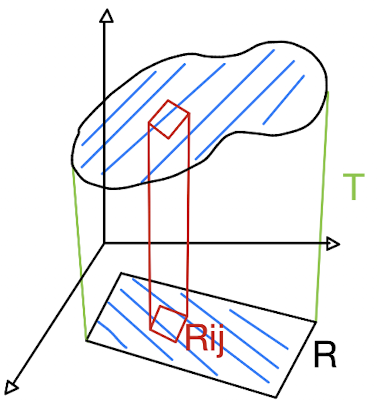
\includegraphics[width=0.35\textwidth]{Analisi2/figures/cilindroide.png}
	\caption{Cilindroide.}
	\label{fig:cilindroide}
\end{figure}

\begin{theorem}\footnote{Slide 19 PDF 24.}\label{th:funzione_continua_integrabile}
	Se $f$ è continua in $R = [a, b]\times [c, d]$ allora è Riemann integrabile.
\end{theorem}

\paragraph{Note sul Teorema:} \begin{itemize}
	\item NON SARÀ FATTA DIMOSTRAZIONE,
	\item È possibile dimostrare il Teorema appena enunciato facendo vedere che la differenza tra somma superiore ed inferiore è minore di $\varepsilon$,
	\item In realtà è sufficiente anche meno affinché una funzione sia integrabile. La classe di funzioni integrabili è più ampia di quella delle funzioni continue e comprende le funzioni con un numero finito di discontinuità, in quanto queste diventano trascurabili. SARANNO TRATTATE SEMPRE FUNZIONI CONTINUE NEL DOMINIO DI INTEGRAZIONE.
\end{itemize} 

\paragraph{Precisazioni:} Se considerate funzioni continue su rettangoli è possibile scrivere automaticamente le formule di riduzione (vedere Teorema \ref{th:riduzione}). Ovvero si calcano due integrali iterativi: prima si integra rispetto ad una variabile e poi rispetto all'altra (applicando il Teorema di riduzione).

\begin{remark}\footnote{Slide 19 PDF 24.}
	Se $f:R=[a,b]\times[c,d]\rightarrow\mathbb{R}$ è del tipo (a variabili separabili) $f(x,y)=g(x)\cdot h(y)$ e supposto che $g\in\mathscrsfs{R}([a,b])$ e $h\in\mathscrsfs{R}([c,d])$ allora$_{\footnotemark}$ $f\in\mathscrsfs{R}(R)$ e
	\begin{equation*}
		\int\int_R f(x,y) dx\,dy=\int^b_a g(x) dx\int^d_c h(y) dy.
	\end{equation*}
\end{remark}

\footnotetext{Se $g$ ed $h$ sono integrabili nei rispettivi intervalli allora $f$, la quale è il prodotto di $g$ e $h$, è integrabile sul prodotto cartesiano $R=[a,b]\times[c,d]$.}

\begin{theorem}[Formula di riduzione]\label{th:riduzione}\footnote{Slide 20 PDF 24.}
	Sia $f:R=[a,b]\times[c,d]\rightarrow\mathbb{R}$ continua in $R$ allora $f$ è integrabile (secondo Riemann) su $R$ (Teorema \ref{th:funzione_continua_integrabile}) e
	\begin{equation}\label{eq:formula_riduzione}
		\int\int_R f(x,y) dx\, dy = \underset{\text{formula a)}}{\int^b_a\left(\int^d_c f(\underset{\text{fissa}}{x},y) dy\right) dx} =\underset{\text{formula b)}}{\int^d_c\left(\int^b_a f(x, \underset{\text{fissa}}{y})dx\right)dy}.
	\end{equation}
\end{theorem}

\paragraph{Cosa significa la formula a) in (\ref{eq:formula_riduzione})?} Quando è integrato rispetto a $y$ significa che la $x$ è fissata, quindi $f$ diventa una funzione di una variabile e dato che $f$ è continua su $[c,d]$ (dato che diventa ad un variabile) allora è integrabile su $[c,d]$. Una volta integrata su $y$ allora $f$ dipende solo da $x$ e dato che $f$ è continua su $[a,b]$ allora è integrabile su questo.

\paragraph{Nota sulla formula di riduzione:} Applicare prima la \textbf{formula a)} e poi la \textbf{formula b)} dipende da com'è fatta $f$.

\begin{example}\footnote{Slide 20 PDF 24.}
	Sia $f(x,y)=x^{-3e^{\frac{y}{x}}}$ su $R=[1, 3]\times[0,1]$. $f$ è continua su $R$, quindi integrabile.
	\paragraph{Formula b):} Tramite la formula b) è più facile trovare una primitiva elementare di $f$.
	\begin{equation*}
		\int_0^1 f(x,y) dy = x\text{ fissata in } [1,3] = \int_0^1 x^{-3} e^{\frac{y}{x}}  dy = x^{-3}\left[x\, e^{\frac{y}{x}}\right]^1_0 =  x^{-3} (x) \left(x\, e^{\frac{1}{x} - x\, e^0}\right) = x^{-2} \left(e^{\frac{1}{x}} - 1\right).
	\end{equation*}
	Quindi,
	\begin{equation*}
		\int\int_R f(x,y) dx\, dy = \int_1^3\left(\int_0^1 f(x,y) dy\right)\, dy = \int_1^3 x^{-2}\left(e^{\frac{1}{x}}-1\right) dx =(\star) 
	\end{equation*}
	ed utilizzando l'integrazione per sostituzione,
	\begin{equation*}
		 \frac{1}{x} = y \;\rightarrow\; dy=\frac{1}{x^2}dx \quad\Longrightarrow\quad \int_1^3e^y -1 dy = \left[e^y-y\right]_1^3 ,
	\end{equation*}
	è ottenuto che
	\begin{equation*}
		(\star) = \left[\frac{1}{x} - e^{\frac{1}{x}}\right]^3_1 = \frac{1}{3} - \sqrt[3]{e}.
	\end{equation*}
\end{example}

\subsection{Domini semplici}
\footnote{Slide 21 PDF 24.} Il caso in cui una funzione integranda $f$ sia definita su un rettangolo è un caso particolare. Se $f$ è definita su un dominio limitato $D\subset\mathbb{R}^2$ (quindi $f$ è limitata), è possibile definire un rettangolo $R=[a,b]\times [c,d]$ opportuno (qualsiasi) tale che $D\subset R$ e ridefinire $f$ in modo tale che sia 0 fuori da $D$. Così facendo è possibile integrare $f$ sul rettangolo e non sul dominio.

\begin{figure}[ht]
	\centering
	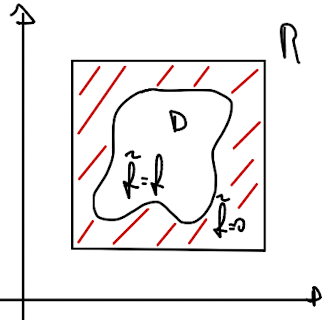
\includegraphics[width=0.35\textwidth]{Analisi2/figures/f_estesa.png}
	\caption{Funzione $f$ estesa.}
	\label{fig:f_estesa}
\end{figure}

\begin{definition}[Funzione integranda estesa da un dominio ad un rettangolo]\footnote{Slide 21 PDF 24.}\label{def:f_estesa_rettangolo}
	Data $f:D\subset R\rightarrow\mathbb{R}$, dove $R=[a,b]\times [c,d]$, è definita $\tilde{f}:R\rightarrow\mathbb{R}$ come segue:
	\begin{equation}\label{eq:f_estesa_rettangolo}
		\tilde{f}(x,y) = 
		\begin{cases}
			f(x,y) & \text{se } (x,y)\in D\\
			0 &\text{altrimenti}
		\end{cases}
	\end{equation}
\end{definition}

\paragraph{Nota su (\ref{eq:f_estesa_rettangolo}):} L'interpretazione geometrica dell'integrale nel caso dell'estensione della funzione non cambia: se considerata al di fuori da $D$ il contributo di $\tilde{f}$ è nullo. $\qed$

\begin{definition}[Integrale secondo Riemann della funzione limitata su un dominio limitato]\label{def:integrale_f_estesa_rettangolo}
	\footnote{Slide 21 PDF 24.} Sia $f:D\subset \mathbb{R}^\rightarrow\mathbb{R}$ limitata su $D$ dominio limitato. Diremo che $f$ è integrabile (secondo Riemann) su $D$ (non rettangolo) se $\tilde f$ (definita come (\ref{eq:f_estesa_rettangolo})) è integrabile (secondo Riemann) su $R$ (rettangolo tale che $D\subset R$) e si pone
	\begin{equation*}
		I(f, D) = \int\int_D f(x,y) dx\, dy = \int \int_R \tilde{f}(x,y) dx\, dy.
	\end{equation*}
\end{definition}

\paragraph{Nota sulla Definizione (\ref{def:integrale_f_estesa_rettangolo}):} La definizione è ben posta e aderisce perfettamente all'interpretazione geometrica dell'integrale doppio di una funzione non negatica come volume di un cilindroide, in quanto l'integrabilità di $f$ nel dominio limitato ed il valore dell'integrale \textbf{\ul{non}} dipendono da $R$ (perché per ogni rettangolo scelto, $f$ vale 0 nei punti fuori da $D$). Inoltre, \textbf{il fatto che $\boldsymbol{f}$ sia limitata è un ipotesi necessaria per la definizione}.$\qed$

\begin{definition}[Area (misura) di Peano-Jordan di una regione del piano]\footnote{Slide 22 PDF 24.}
	Un sottoinsieme (nel piano) limitato $D\subset\mathbb{R}^2$ si dice misurabile secondo Peano-Jordan se la funzione $f(x,y)\equiv 1$ è integrabile (secondo Riemann) su $D$. In tal caso, l'Area ($\slash$ misura) di $D$ è definita come
	\begin{equation}\label{eq:area_p-j_regione_piano}
		Area(D) = |D| =\int\int_D 1 dx\, dy,
	\end{equation}
	se ha senso (ovvero è un numero finito).
\end{definition}

\paragraph{$\boldsymbol{D}$ misurabile:} $D$ si dice misurabile se ha misura finita, quindi se (\ref{eq:area_p-j_regione_piano}) è un numero finito.

\begin{example}
	$R= [a,b]\times [c,d]$ è (limitato e) misurabile secondo P-J e 
	\begin{equation*}
		|R| =\int \int_R 1 dx\, dy = \int_a^b\int_c^d 1 dx\, dy = (b-a) (d-c).
	\end{equation*}
\end{example}

\paragraph{Deduduzioni sulla misura di Peano-Jordan:} Tutti gli insiemi che conosciuti della geometria elementare (cerchi, poligoni, quadrati, rettangoli, ecc.) sono misurabili e la loro misura è l'area elementare (quindi, in questo caso, misura ed area coincidono).

\begin{example}[Dominio limitato non misurabile secondo Peano-Jordan]
	\footnote{Slide 23 PDF 24.} Sia $Q = [0,1]\times[0,1]$ insieme limitato con entrambe le coordinate razionali, è definita la funzione di Dirichlet come
	\begin{equation*}
		f(x,y) =
		\begin{cases}
			1, &\text{se } (x,y)\in Q \text{ e } (x,y)\in\mathbb{Q}\\
			0 &\text{altrimenti}
		\end{cases}
	\end{equation*}
	La funzione caratteristica $f(x,y) \equiv 1$ (relativa al dominio) non è Riemann integrabile su $Q$ e non è misurabile secondo P-J.
\end{example}

\paragraph{Nota:} I domini semplici sono Reamann integrabili (?) in quanto sono limitati compresi fra il grafico di due funzioni continue e due rette verticali opportunamente prese.

\subsection{Proprietà degli integrali doppi}
\footnote{Slide 25 PDF 25.}
\begin{property}
	 Sia $D\subset\mathbb{R}^2$ insieme limitato e misurabile:
	\begin{enumerate}
		\item \textbf{Linearità:} Se $f,g\in\mathscrsfs{R}(D)$ e se $\alpha,\beta\in \mathbb{R}$ \textbf{\ul{allora}} $\alpha f + \beta g\in \mathscrsfs{R}(D)$ e
		\begin{equation*}
			\int\int_D [\alpha f(x,y) + \beta g(x,y)]dx\, dy = \alpha\int\int_D \alpha f(x,y) dx\, dy + \beta\int\int_D \beta g(x,y)dx\, dy.
		\end{equation*}
		\item \textbf{Monotonia (dell'integrale rispetto all'integranda):} Se $f,g\in\mathscrsfs{R}(D)$ e se $f\leq g$ su $D$ \textbf{\ul{allora}}
		\begin{equation*}
			\int\int_D f(x,y) dx\, dy \leq \int\int_D g(x,y) dx\, dy.
		\end{equation*}
		\item \textbf{Monotonia (dell'integrale rispetto all'integranda) - 2:} Se $f\in \mathscrsfs{R}(D)$ allora $|f|\in\mathscrsfs{R}(D)$\footnote{Ovvero $|f|$ è Riemann integrabile, quindi vale $\int\int_D |f(x,y)| dx\, dy$.} ed in particolare vale
		\begin{equation*}
			\left| \int\int_D f(x,y) dx\, dy\right| \leq \int\int_D |f(x,y)| dx\, dy.
		\end{equation*}
	\end{enumerate}
\end{property}

\subsection{Integrazione su domini (regioni) semplici misurabili secondo Peano-Jordan}
\footnote{Slide 25 PDF 24.} È necessario specificare su quale dominio è operata l'integrazione (ad esempio per applicare al meglio la formula di riduzione).

Date la Definizione \ref{def:f_estesa_rettangolo} di funzione estesa su un rettangolo e la Definizione \ref{def:integrale_f_estesa_rettangolo} di Integrale secondo Riemann della funzione limitata su un dominio limitato, non ci aiutano con il calcolo integrale perché anche se è considerata una funzione $f$ continua su $D$ non è detto che una la sua estensione $\tilde{f}$ sia continua \footnote{Quando è considerata l'estensione di $f$ continua su $D$, in genere, non è ottenuta un'estensione continua e quindi non è possibile applicare la formula di riduzione (per problemi, anche sulla frontiera del dominio).}.
Pertanto, è necessario estendere la classe delle funzioni sulle quali è possibile operare l'integrazione e utilizzare una formula di riduzione, la quale varrà per insiemi diversi dai rettangoli. Questi nuovi insiemi sono chiamati domini semplici, in particolare saranno considerate la loro unione quando avranno parte delle rispettive frontiere in comune. In questo modo è possibile applicare la formula di additività  rispetto al dominio di integrazione (il dominio grande è spezzettato in domini semplici con parte della frontiera in comune) e di conseguenza l'integrale doppio sul dominio "generale" sarà una somma di integrali doppi su domini semplici.\\
È necessario definire cosa siano i domini semplici, i quali sono definibili come regioni misurabili secondo Peano-Jordan.

\begin{definition}[Regione y-semplice]\footnote{Slide 26 PDF 25.}
	
\end{definition}